\chapter{Implementacija i korisničko sučelje}
		
		
		\section{Korištene tehnologije i alati}
		
			%\textbf{\textit{dio 2. revizije}}
			
			 %\textit{Detaljno navesti sve tehnologije i alate koji su primijenjeni pri izradi dokumentacije i aplikacije. Ukratko ih opisati, te navesti njihovo značenje i mjesto primjene. Za svaki navedeni alat i tehnologiju je potrebno \textbf{navesti internet poveznicu} gdje se mogu preuzeti ili više saznati o njima}.
			 
			 Za ostvarenje komunikacije između članova projektnog tima korištena je aplikacija WhatsApp\footnote{https://www.whatsapp.com/}. Za održavanje sastanaka unutar tima korištena je platforma MS Teams\footnote{https://www.microsoft.com/microsoft-teams/}. Komunikacija s demonstratorom i asistentom ostvarena je također s pomoću platforme MS Teams. Praćenje napretka i raspodjela zadataka u timu ostvarena je pomoću alata Jira\footnote{https://www.atlassian.com/software/jira}. Jira pomoću tzv. issue nudi pogućnost podijele izrade u manje zadatke koji se zatim mogu pridijeliti nekom od članova tima. Svaki od člana tima zatim može za svaki zadatak prikazati u kojoj je fazi izrade što ostalim članovima nudi mogućnost uvida u to na čemu drugi članovi tima trenutno rade. Upravljanje izvornim kodom i dokumentacijom ostvareno je s pomoću alata Git\footnote{https://git-scm.com/}. Udaljeni repozitorij pohranjen je na platformi GitHub\footnote{https://github.com/}. Za izradu dokumentacije projekta korišten je LaTeX\footnote{https://www.latex-project.org/}. UML dijagram obrazaca uporabe, sekvencijski dijagram, prva revizija dijagrama razreda, dijagram aktivnosti, dijagram stanja, dijagram komponenti i dijagram razmještaja napravljeni su s pomoću alata Astah UML\footnote{https://astah.net/products/astah-uml/}. Implementacijski dijagram razreda napravljen je s pomoću alata IntelliJ IDEA\footnote{https://www.jetbrains.com/idea/}. Model baze podataka izgrađen je alatom ERDPlus\footnote{https://erdplus.com/}. Za izradu backend dijela aplikacije korišten je radni okvir Java\footnote{https://www.java.com/en/} Spring\footnote{https://spring.io/}, a za razvoj na backendu korišteno je razvojno okruženje IntelliJ IDEA. Za izradu frontend dijela aplikacije korištena je knjižnica React\footnote{https://react.dev/} uz programski jezik TypeScript\footnote{https://www.typescriptlang.org/}. Za ispitivanje sustava korišteni su JUnit\footnote{https://junit.org/} i Selenium\footnote{https://www.selenium.dev/}. Za puštanje aplikacije u pogon korištena je platforma Render\footnote{https://render.com/}.
			
			
			\eject 
		
	
		\section{Ispitivanje programskog rješenja}

			\subsection{Ispitivanje komponenti}
			
						\subsection{Testiranje Gettera i Settera}
			
			TestGettersAndSetters služi za provjeru ispravnosti gettera i settera za klasu \texttt{Account}. U ovom testu se inicijalizira objekt \texttt{Account} s određenim podacima (email, ime, prezime, lozinka, i uloga), a zatim se koriste getteri za dohvaćanje tih podataka i setteri za postavljanje novih vrijednosti. Nakon postavljanja novih vrijednosti, ponovno se koriste getteri za provjeru je li objekt uspješno promijenjen prema očekivanjima.
			
			\begin{lstlisting}
				@Test
				public void testGettersAndSetters() {
					Account account = new Account("test@example.com", "John", "Doe", "password", Roles.USER);
					
					Assertions.assertEquals("test@example.com", account.getEmail());
					Assertions.assertEquals("John", account.getFirstName());
					Assertions.assertEquals("Doe", account.getLastName());
					Assertions.assertEquals("password", account.getPassword());
					Assertions.assertEquals(Roles.USER, account.getRole());
					
					account.setEmail("newemail@example.com");
					account.setFirstName("Jane");
					account.setLastName("Smith");
					account.setPassword("newpassword");
					account.setRole(Roles.ADMIN);
					
					Assertions.assertEquals("newemail@example.com", account.getEmail());
					Assertions.assertEquals("Jane", account.getFirstName());
					Assertions.assertEquals("Smith", account.getLastName());
					Assertions.assertEquals("newpassword", account.getPassword());
					Assertions.assertEquals(Roles.ADMIN, account.getRole());
				}
			\end{lstlisting}
			
			\subsection{Testiranje Token Verzije}
			
			TestTokenVersion provjerava funkcionalnost metoda za rad s token verzijom (\texttt{getTokenVersion()}, \texttt{incrementTokenVersion()}, \texttt{setTokenVersion()}) za klasu \texttt{Account}. Prvo se inicijalizira objekt \texttt{Account}, a zatim se provjerava da li je početna vrijednost token verzije jednaka 0. Nakon toga, koristi se metoda \texttt{incrementTokenVersion()} za povećanje verzije za 1 i provjerava se da li je nova vrijednost 1. Također se koristi metoda \texttt{setTokenVersion()} za postavljanje verzije na 5 i provjerava se je li postavljena vrijednost ispravna.
			
			\begin{lstlisting}
				@Test
				public void testTokenVersion() {
					Account account = new Account("test@example.com", "John", "Doe", "password", Roles.USER);
					
					Assertions.assertEquals(0L, account.getTokenVersion());
					
					account.incrementTokenVersion();
					Assertions.assertEquals(1L, account.getTokenVersion());
					
					account.setTokenVersion(5L);
					Assertions.assertEquals(5L, account.getTokenVersion());
				}
			\end{lstlisting}
			
			\subection{Testiranje Metode \texttt{toString()}}
			
			ToString test provjerava da li metoda \texttt{toString()} klase \texttt{Account} vraća očekivani format teksta. Prvo se inicijalizira objekt \texttt{Account} s određenim podacima, a zatim se koristi metoda \texttt{toString()} za dobivanje string reprezentacije objekta. Očekivana string reprezentacija se uspoređuje s unaprijed definiranom očekivanom vrijednošću.
			
			\begin{lstlisting}
				@Test
				public void testToString() {
					Account account = new Account("test@example.com", "John", "Doe", "password", Roles.USER);
					
					String expectedToString = "Account{" +
						"id=null" +
						", email='test@example.com'" +
						", firstName='John'" +
						", lastName='Doe'" +
						", password='password'" +
						", role=USER" +
						", tokenVersion=0" +
						'}';
					
					Assertions.assertEquals(expectedToString, account.toString());
				}
			\end{lstlisting}
			
			\subsection{Testiranje Metode \texttt{testLoadUserByUsername_ThrowsException()}}
			
			Koristi se Assertions.assertThrows iz JUnit frameworka kako bi se provjerilo da će poziv loadUserByUsername(email) metode iz accountUserDetailsService doista izazvati iznimku tipa UsernameNotFoundException. Očekuje se da metoda loadUserByUsername baci iznimku kada korisnik s navedenim emailom ne postoji u sustavu.
			
			\begin{lstlisting}
				@Test
				public void testLoadUserByUsername_ThrowsException() {
					String email = "test@example.com";
					
					when(accountService.findByEmail(email)).thenReturn(Optional.empty());
					
					Assertions.assertThrows(UsernameNotFoundException.class, () -> {
						accountUserDetailsService.loadUserByUsername(email);
					});
				}
			\end{lstlisting}
			
			\subsection{Testiranje Metode \texttt{testGetAllDicts_EmptyList()}}	
			
			\begin{itemize}
				\item \textbf{Arrange}: Postavlja se ponašanje mock objekta \texttt{dictionaryService} kako bi simulirali situaciju kada nema rječnika. Očekujemo da će \texttt{dictionaryService.getAllDicts()} vratiti praznu listu koristeći \texttt{when} metodu.
				
				\item \textbf{Act}: Poziva se \texttt{GET()} metoda iz \texttt{dictionaryController} kako bi se dobio odgovor.
				
				\item \textbf{Assert}: Provjerava se da li je odgovor tipa \texttt{HttpStatus.NOT\_FOUND} (404), što označava da nema dostupnih rječnika. Također se provjerava da li je tijelo odgovora prazna lista (\texttt{Collections.emptyList()}).
				
				\item \textbf{Verify}: Koristi se \texttt{verify} kako bi se provjerilo da je \texttt{dictionaryService.getAllDicts()} pozvana točno jednom i da nije bilo više interakcija s tim servisom (\texttt{verifyNoMoreInteractions(dictionaryService)}).
			\end{itemize}
			
			\begin{lstlisting}
				
				@Test
				public void testGetAllDicts_EmptyList() {
					// Arrange
					when(dictionaryService.getAllDicts()).thenReturn(Collections.emptyList());
					
					// Act
					ResponseEntity<List<Dictionary>> response = dictionaryController.GET();
					
					// Assert
					Assertions.assertEquals(HttpStatus.NOT_FOUND, response.getStatusCode());
					Assertions.assertEquals(Collections.emptyList(), response.getBody());
					
					verify(dictionaryService, times(1)).getAllDicts();
					verifyNoMoreInteractions(dictionaryService);
				}
				
			\end{lstlisting}
			
			\subsection{Testiranje Metode \texttt{testGetAllDicts_NonEmptyList()}}	
			
			\begin{itemize}
				\item \textbf{Arrange}: Postavlja se ponašanje mock objekta \texttt{dictionaryService} kako bi simulirali situaciju kada lista rječnika sadrži nekoliko rječnika. Očekujemo da će \texttt{dictionaryService.getAllDicts()} vratiti listu rječnika koristeći \texttt{when} metodu.
				
				\item \textbf{Act}: Poziva se \texttt{GET()} metoda iz \texttt{dictionaryController} kako bi se dobio odgovor.
				
				\item \textbf{Assert}: Provjerava se da li je odgovor tipa \texttt{HttpStatus.OK} (200), što označava uspješan zahtjev, te da li tijelo odgovora sadrži listu rječnika koja je vraćena iz \texttt{dictionaryService}.
				
				\item \textbf{Verify}: Koristi se \texttt{verify} kako bi se provjerilo da je \texttt{dictionaryService.getAllDicts()} pozvana točno jednom i da nije bilo više interakcija s tim servisom (\texttt{verifyNoMoreInteractions(dictionaryService)}).
			\end{itemize}
			
			\begin{lstlisting}
				
				@Test
				public void testGetAllDicts_NonEmptyList() {
					// Arrange
					List<Dictionary> dictionaries = List.of(new Dictionary(), new Dictionary());
					when(dictionaryService.getAllDicts()).thenReturn(dictionaries);
					
					// Act
					ResponseEntity<List<Dictionary>> response = dictionaryController.GET();
					
					// Assert
					Assertions.assertEquals(HttpStatus.OK, response.getStatusCode());
					Assertions.assertEquals(dictionaries, response.getBody());
					
					verify(dictionaryService, times(1)).getAllDicts();
					verifyNoMoreInteractions(dictionaryService);
				}
				
			\end{lstlisting}

			\subsection{Ispitivanje sustava}
			
			 \textit{Potrebno je provesti i opisati ispitivanje sustava koristeći radni okvir Selenium\footnote{\url{https://www.seleniumhq.org/}}. Razraditi \textbf{minimalno 4 ispitna slučaja} u kojima će se ispitati redovni slučajevi, rubni uvjeti te poziv funkcionalnosti koja nije implementirana/izaziva pogrešku kako bi se vidjelo na koji način sustav reagira kada nešto nije u potpunosti ostvareno. Ispitni slučaj se treba sastojati od ulaza (npr. korisničko ime i lozinka), očekivanog izlaza ili rezultata, koraka ispitivanja i dobivenog izlaza ili rezultata.\\ }
			 
			 \textit{Izradu ispitnih slučajeva pomoću radnog okvira Selenium moguće je provesti pomoću jednog od sljedeća dva alata:}
			 \begin{itemize}
			 	\item \textit{dodatak za preglednik \textbf{Selenium IDE} - snimanje korisnikovih akcija radi automatskog ponavljanja ispita	}
			 	\item \textit{\textbf{Selenium WebDriver} - podrška za pisanje ispita u jezicima Java, C\#, PHP koristeći posebno programsko sučelje.}
			 \end{itemize}
		 	\textit{Detalji o korištenju alata Selenium bit će prikazani na posebnom predavanju tijekom semestra.}
			
			\eject 
		
		
		\section{Dijagram razmještaja}
			
			%\textbf{\textit{dio 2. revizije}}
			
			 %\textit{Potrebno je umetnuti \textbf{specifikacijski} dijagram razmještaja i opisati ga. Moguće je umjesto specifikacijskog dijagrama razmještaja umetnuti dijagram razmještaja instanci, pod uvjetom da taj dijagram bolje opisuje neki važniji dio sustava.}
			 
			 \begin{figure}[H]
			 	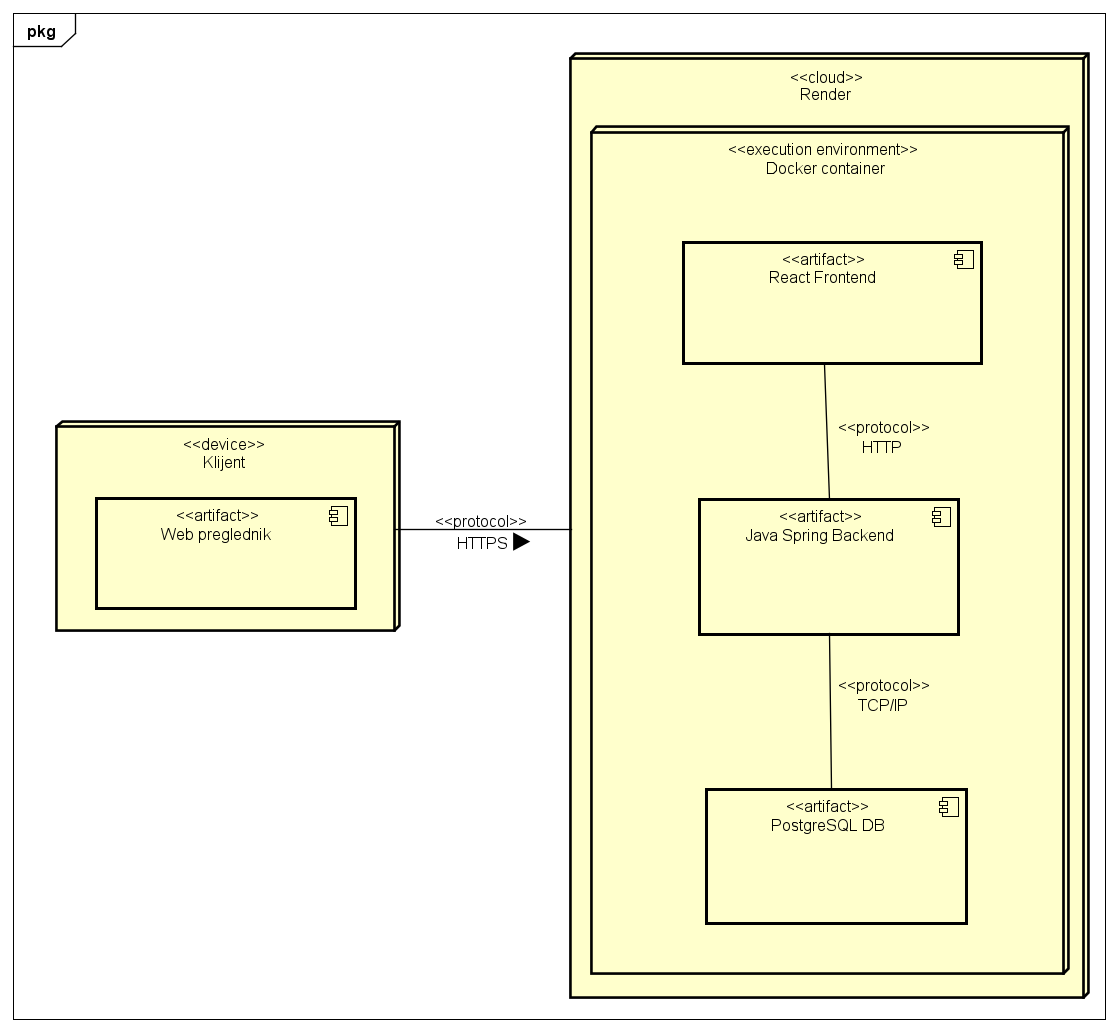
\includegraphics[width=\textwidth]{slike/DeploymentDiagram.PNG}
			 	\caption{Dijagram razmještaja}
			 	\label{fig:deploymentDiagram}
			 \end{figure}
			 
			 \newpage
			 
			 Slika 5.1 prikazuje dijagram razmještaja. Dijagram razmještaja prikazuje raspodjelu programskih komponenti kao što su izvršne datoteke i virtualna izvršna okruženja. Dijagram se sastoji od dvaju glavnih čvorova nazvanih Klijent i Render. Čvor Klijent predstavlja uređaj kojim klijent, odnosno korisnik pokušava pristupiti sustavu. Čvor se sastoji od jednog artefakta, Web preglednika. Web preglednik je izvršna datoteka kojom korisnik šalje sve zahtjeve u sustav i prima odgovore iz sustava. Drugi čvor na dijagramu je Render. Render je poslužiteljsko računalo/a koja su smještena u oblaku. Cijela aplikacija je smještena unutar kontejnera Docker u oblaku Render. Kontejner Docker je virtualno izvršno okruženje. Pripadni čvor Docker container je ugniježđen unutar čvora Render. Frontend dio aplikacije implementiran je kao React aplikacija, backend dio implementiran je koristeći Java Spring radni okvir, a baza podataka koja služi da pohranu svih potrebnih podataka implementirana je kao PostgreSQL. Komunikacija između korisnika, odnosno web preglednika i aplikacije odvija se preko HTTPS protokola, protokola na aplikacijskom sloju. Svaki od artefakata koji zajedno čine aplikaciju, međusobno komuniciraju. Komunikacija između frontend i backend dijela aplikacije izvodi se preko HTTP protokola, dok se komunikacija između Java Spring backenda i baze podataka izvodi s pomoću protokola nižih slojeva, točnije TCP/IP protokolima.
			
			\eject 
		
		\section{Upute za puštanje u pogon}
		
			\textbf{\textit{dio 2. revizije}}\\
		
			 \textit{U ovom poglavlju potrebno je dati upute za puštanje u pogon (engl. deployment) ostvarene aplikacije. Na primjer, za web aplikacije, opisati postupak kojim se od izvornog kôda dolazi do potpuno postavljene baze podataka i poslužitelja koji odgovara na upite korisnika. Za mobilnu aplikaciju, postupak kojim se aplikacija izgradi, te postavi na neku od trgovina. Za stolnu (engl. desktop) aplikaciju, postupak kojim se aplikacija instalira na računalo. Ukoliko mobilne i stolne aplikacije komuniciraju s poslužiteljem i/ili bazom podataka, opisati i postupak njihovog postavljanja. Pri izradi uputa preporučuje se \textbf{naglasiti korake instalacije uporabom natuknica} te koristiti što je više moguće \textbf{slike ekrana} (engl. screenshots) kako bi upute bile jasne i jednostavne za slijediti.}
			
			
			 \textit{Dovršenu aplikaciju potrebno je pokrenuti na javno dostupnom poslužitelju. Studentima se preporuča korištenje neke od sljedećih besplatnih usluga: \href{https://aws.amazon.com/}{Amazon AWS}, \href{https://azure.microsoft.com/en-us/}{Microsoft Azure} ili \href{https://www.heroku.com/}{Heroku}. Mobilne aplikacije trebaju biti objavljene na F-Droid, Google Play ili Amazon App trgovini.}
			
			
			\eject 